\chapter{Theoretical Background}
\section{Basics in Modeling Light in Computer Graphics}

\subsection{Radiometry}
One purpose of Computer Graphics is to simulate the interaction of light on a surface and how a real-world observer, such as a human eye, will perceive this. These visual sensations of an eye are modeled relying on a virtual camera which captures the emitted light from the surface. The physical basis to measure such reflected light depicts radiometry which is about measuring the electromagnetic radiation transfered from a soruce to a receiver. 

Fundamentally, light is a form of energy propagation, consisting of a large collection of photons, whereat each photon can be considered as a quantum of light that has a position, direction of propagation and a wavelength $\lambda$. A photon travels at a certain speed $v = \frac{c}{n}$, that depends only the speed of light $c$ and the refractive index $n$ through which it progrates. Its frequency is defined by $f = \frac{v}{\lambda}$ and its carried amount of energy $q$, mearsured in the SI unit Joule, is given by $q = hf= \frac{hv}{\lambda n}$ where $h$ is the Plank's constant. The total energy of a large collection of photons is hence $Q = \sum_i q_i$.

\subsection{Spectral Energy}

It is important to understand that the human eye is not equally sensitive to all wavelength of the spectrum of light and therefore responds differently to specific wavelengths. Remember that our goal is to model the human visual perception. This is why we consider the energy distribution of a light spectrum rather than considering the total energry of a photon collection since then we could weight the distribution according the human visual system. So the question we want to answer is: How is the energy distributed across wavelengths of light?

The idea is to make an energy histrogram from a given photon collection. For this we have to order all photons by their associated wavelength, discretize wavelength spectrum, count all photons which then will fall in same wavelength-interval, and then, finally, normalize each interval by the total energy $Q$. This will give us a histogram which tells us the spectral energy $Q_{\lambda}$ for a given discrete $\lambda$ interval and thus models the so called spectral energy distribution $\footnote{Intensive quantities can be thought of as density functions that tell the density of an extensive quantity at an infinitesimal point.}$.

\subsection{Spectral Power}
Rendering an image in Computer Graphics corresponds to capturing the color sensation of an illuminated, target scene at a certain point in time. As previousely seen, each color is associated by a wavelength and is directly related to a certain amount of enegry. In order to determine the color of a to-be-rendered pixel of an image, we have to get a sense of how much light (in terms of energy) passes through the area which the pixel corresponds to. One possibility is to consider the flow of energy $\Phi = \frac{\Delta Q}{\Delta t}$ transferred through this area over a small period of time. This allows us to measure the energy flow through a pixel during a certain amount of time. 

In general, power is the estimated rate of energy production for light sources and corresponds to the flux. It is measured in the unit Watts, denoted by Q. Since power is a rate over time, it is well defined even when energy production is varying over time. As with Spectral Energy for rendering, we are really interested in the spectral power $\Phi_\lambda = \frac{\Phi}{\lambda}$, measured in Watts per nanometer.

\subsection{Spectral Irradiance}
Before we can tell how much light is reflected from a given point on a surface towards the viewing direction of an observer, we first have to know how much light arrives at this point. Since in general a point has no length, area or even volume associated, let us instead consider an infinitimal area $\Delta A$ around a such a point. Then, we can ask ourself how much light falls in such a small area. When further observing this process over a short period in time, this quantity is the spectral irradiance $E$ as illustrated in figure $\ref{fig:irradiance}$. Summarized, this quantity tells us how much spectral power is incident on a surface per unit area and mathematically is equal:

\begin{equation}
 E = \frac{\Phi_{\lambda}}{\Delta A}
\end{equation} 

\begin{figure}[H]
  \centering
  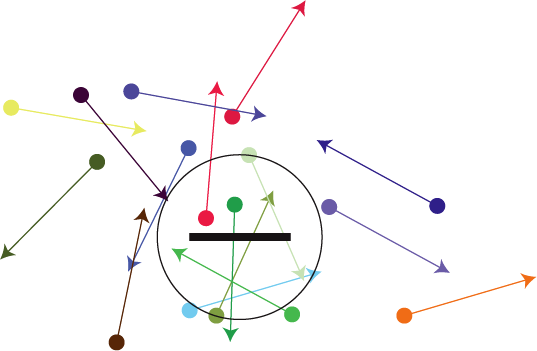
\includegraphics[scale=0.5]{background/irradiance.png}
  \caption{Irradiance is the summed up radiance over all directions}
  \label{fig:irradiance}
\end{figure}

\subsection{Spectral Radiance}
When rendering an image we have to determine the color of each pixel of the image. Although irradiance tells us how much light is arriving at a point as illustrated in figure $\ref{fig:irradiance}$, it tells us little about the direction that light comes from. This relates to how the human eye perceives the brightness of an illuminated objects when looking at it in a certain direction. 

\begin{figure}[H]
  \centering
  \subfigure[Radiance is photon ray density number of photons per area per solid angle.]{
    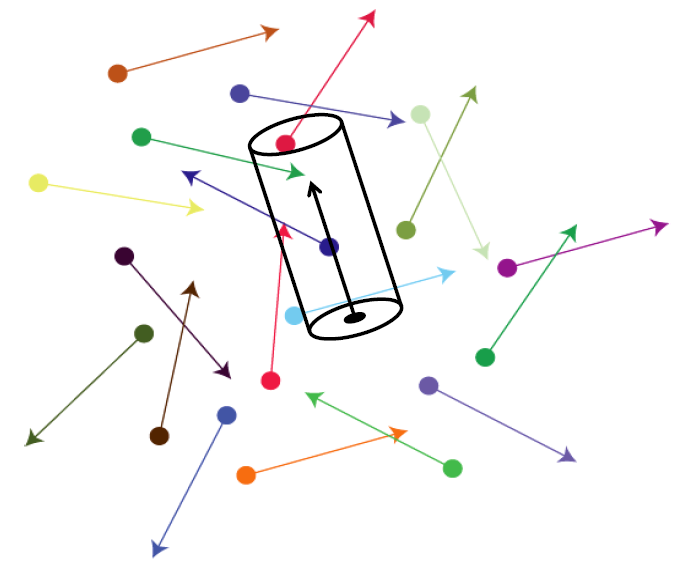
\includegraphics[scale=0.3]{background/radiance.png}
    \label{fig:radiance}
  }
~
  \subfigure[Solid angle is the area of a surface patch on a unit sphere which is spanned by a set of directions]{
    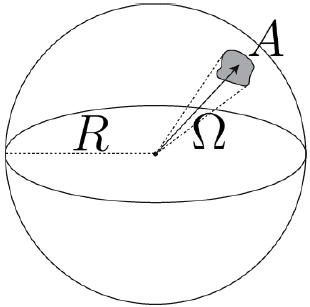
\includegraphics[scale=0.5]{background/solidangle.png}
    \label{fig:solidangle}
  }

\label{fig:radianceBasics}
\end{figure}

This concepted is described by the radiometric quantity radiance. This is basically a measure of light energy passing through or is emitted off from a small area around a point on a surface towards a given direction during a short period in time. More formally this is the spectral power emerging from an arbitrary point (an infinitimal area around this point) and falls within a given solid angle in specific direction (usually towards the observer) as shown in figure $\ref{fig:radiance}$. Formally, this leads us to the following mathematical formalism: 

\begin{equation}
 L_{\lambda}(\omega) = \frac{d^2 \Phi_{\lambda}}{dA d\Omega} \approx \frac{\Phi_{\lambda}}{\Omega A}
\end{equation}

where $L$ is the observed radiance in the unit energy per unit area per solid angle, which is $Wm^-2 sr^-1$ in direction $\omega$ which has an angle $\theta$ between the surface normal and $\omega$, $\Theta$ is the total flux or power emitted, $\theta$ is the angle between the surface normal and the specified direction, $A$ is the area of the surface and $\Omega$ is the solid angle in the unit steradian subtended by the observation or measurement.

It is useful to distinguish between radiance incident at a point on a surface and excitant from that point. Terms for these concepts sometimes used in the graphics literature are surface radiance $L_r$ for the radiance \textit{reflected} from a surface and field radiance $L_i$ for the radiance \textit{incident} at a surface.  

\subsection{BRDF}
In order to render the colorization of an observed object, a natural question in computer graphics is what portion of the reflected, incident light a viewer will receive, when he looks at an illuminated object. Therefore for any given surfaces which is illuminated from a certain direction $\omega_i$, we can ask ourself how much light is reflected off of any point on this surface towards a viewing direction $\omega_r$. This is where the Bidirectional Reflectance Distribution Function (short: BRDF) comes into play, which is a radiometric quantity telling us how much light is reflected at an opaque surface. Mathematically speaking, the BRDF is the ratio of the reflected radiance pointing to the direction $\omega_r$ to the incident irradiance comming from the inverse direction of $\omega_i$ as illustrated in figure $\ref{fig:brdfillustration}$. 

\begin{figure}[ht]
  \centering
  
\includegraphics[scale=0.25]{brdfdiagram.png}
  \caption[brdfillustration]{Illistration$\footnotemark$ of the BRDF model, where $\omega_i$ is pointing to the light source and the existing direction is denoted by $\omega_r$. Both direction unit direction vectors defined w.r.t to a surface normal $\mathbf{n}$ for every point on the surface.}
  \label{fig:brdfillustration}  
\end{figure}
\footnotetext{image of illustration has been taken from \href{http://en.wikipedia.org/wiki/Bidirectional_reflectance_distribution_function}{wikipedia}}

Which formally is for any given wavelength $\lambda$ equivalent to:

\begin{align}
  BRDF_{\lambda}(\omega_i, \omega_r)
  & = \frac{dL_r(\omega_r)}{dE_i(\omega_i)} \nonumber \\
  & = \frac{dL_r(\omega_r)}{L_i(\omega_i)cos(\theta_i)d\omega_i}
  \label{eq:defbrdf}
\end{align}

Where $L_{r}$ is the reflected radiance, $E_i$ is the irradiance and $\theta_{\text{i}}$ is the angle between $\omega_{\text{i}}$ and the surface normal $\mathbf n$. 

\subsection{Colorspace}

\subsection{Spectral Rendering}





\section{Wave Theory for Light and Diffraction}




\section{Stam's BRDF formulation}
\label{sec:sumstam}
In his paper about Diffraction Shader, J. Stam derives a BRDF which is modeling the effect of diffraction for various analytical anisotropic reflexion models relying on the so called scalar wave theory of diffraction for which a wave is assumed to be a complex valued scalar. 
It's noteworthy, that Stam's BRDF formulation does not take into account the polarization of the light. Fortunately, light sources like sunlight and light bulbs are unpolarized. 

A further assumption in Stam's Paper is, the emanated waves from the source are stationary, which implies the wave is a superposition of independent monochromatic waves. This implies that each wave is associated to a definite wavelength lambda. However, sunlight once again fulfills this fact.

In our simulations we will always assume we have given a directional light source, i.e. sunlight. Hence, Stam's model can be used for our derivations.

For his derivations Stam uses the Kirchhoff integral (ADD REF TO WIKI), which is relating the reflected field to the incoming field. This equation is a formalization of Huygen’s well-known principle that states that if one knows the wavefront at a given moment, the wave at a later time can be deduced by considering each point on the first wave as the source of a new disturbance. Mathematically speaking, once the field  $\psi_1 =  e^{ik\mathbf{x} \cdot \mathbf{s}\mathbf{s}}$ on the surface is known, the field $\psi_2$ everywhere else away from the surface can be computed.
More precisely, we want to compute the wave $\psi_2$ equal to the reflection of an incoming planar monochromatic wave $\psi_1 = e^{ik \omega_i * x}$  traveling in the direction $\omega_i$ from a surface $S$ to the light source. Formally, this can be written as:

\begin{equation}
\psi_{2}(\omega_i, \omega_r) = \frac{i k e^{i K R}}{4 \pi R} (F(-\omega_i-\omega_r)-(-\omega_i+\omega_r)) \cdot I_{1}(\omega_i, \omega_r) 
\label{eq:kirchhoff}
\end{equation}

with

\begin{equation}
I_{1}(\omega_i, \omega_r) = \int_{S} \hat{\mathbf{n}} e^{ik(-\omega_i-\omega_{r}) \cdot \mathbf{s} d\mathbf{s}}
\label{eq:IBase}
\end{equation}

In applied optics, when dealing with scattered waves, one does use differential scattering cross-section rather than defining a BRDF which has the following identity: 

\begin{equation}
    \sigma^0 = 4 \pi \lim_{R \to \infty} R^2 \frac{\langle \left|\psi_2\right|^2\rangle}{\langle \left|\psi_1\right|^2\rangle}
\end{equation}

where R is the distance from the center of the patch to the receiving point $x_p$, $\hat{\mathbf{n}}$ is the normal of the surface at s and the vectors:

The relationship between the BRDF and the scattering cross section can be shown to be equal to 

\begin{equation}
 BRDF = \frac{1}{4\pi}\frac{1}{A}\frac{\sigma^0}{cos(\theta_i)cos(\theta_r)}
 \label{fig:crossscateringbrdfrelationship} 
\end{equation}

where $\theta_i$ and $\theta_r$ are the angles of incident and reflected directions on the surface with the surface normal $n$. See ~\ref{fig:geometricsetup}.

\begin{figure}[ht]
  \centering
  
\includegraphics[scale=0.25]{brdfdiagram.png}
  \caption{$\omega_i$ points toward the light source, $\omega_r$ points toward the camera, $n$ is the surface normal}
  \label{fig:geometricsetup}  
\end{figure}

The components of vector resulting by the difference between these direction vectors:
In order to simplify the calculations involved in his vectorized integral equations, Stam considers the components of vector 
\begin{equation}
  (u,v,w) = -\omega_i - \omega_r 
\label{eq:uvw}
\end{equation}

explicitly and introduces the equation: 
\begin{equation}
  I(ku,kv) = \int_{S} \hat{\mathbf{n}} e^{ik(u,v,w) \cdot \mathbf{s} d\mathbf{s}} 
\label{eq:Istart}
\end{equation}

which is a first simplification of $\ref{eq:IBase}$. Note that the scalar $w$ is the third component of ~\ref{eq:uvw} and can be written as $w = -(cos(\theta_i)+cos(\theta_r))$ using spherical coordinates. The scalar $k=\frac{2\pi}{\lambda}$ represent the wavenumber.


During his derivations, Stam provides a analytical representation for the Kirchhoff integral assuming that each surface point $s(x,y)$ can be parameterized by $(x,y,h(x,y))$ where $h$ is the height at the position $(x,y)$ on the given $(x,y)$ surface plane. Using the tangent plane approximation for the parameterized surface and plugging it into $\ref{eq:Istart}$ he will end up with: 

\begin{equation}
    \mathbf{I}(ku, kv) = \int \int (-h_{x}(x,y), -h_{y}(x,y), 1) e^{ikwh(x,y)} e^{ik(ux + vy)} dx dy
\label{eq:I1}
\end{equation}

For further simplification Stam formulates auxillary function which depends on the provided height field: 
\begin{equation}
  p(x,y) = e^{iwkh(x,y)} 
\label{eq:px}
\end{equation}

which will allow him to further simplify his equation $\ref{eq:I1}$ to:

\begin{equation}
    \mathbf{I}(ku, kv) = \int \int \frac{1}{ikw}(-p_x, -p_y, ikwp) dx dy
\label{eq:I2}
\end{equation}

where he used that $(-h_{x}(x,y), -h_{y}(x,y), 1)e^{kwh(x,y)}$ is equal to $\frac{(-p_x, -p_y, ikwp)}{ikw}$ using the definition of the partial derivatives applied to the function $\ref{eq:px}$.

Let $P(x,y)$ denote the Fourier Transform (FT) of $p(x,y)$. Then, the differentiation with respect to x respectively to y in the Fourier domain is equivalent to a multiplication of the Fourier transform by $-iku$ or $-ikv$ respectively. This leads him to the following simplification for $\ref{eq:I1}$:

\begin{equation}
    \mathbf{I}(ku, kv) = \frac{1}{w}P(ku, kv) \cdot (u,v,w)
\label{eq:I3}
\end{equation}

Let us consider the term $g = (F(-\omega_i - \omega_r)-(-\omega_i + \omega_r))$, which is a scalar factor of $\ref{eq:kirchhoff}$. The dot product with $g$ and $(-\omega_i - \omega_r)$ is equal $2F(1 + \omega_i \cdot \omega_r)$. Putting this finding and the identity $\ref{eq:I3}$ into $\ref{eq:kirchhoff}$ he will end up with:

\begin{equation}
\psi_{2}(\omega_i, \omega_r) = \frac{i k e^{i K R}}{4 \pi R} \frac{2F(1 + \omega_i \cdot \omega_r)}{w} P(ku, kv)
\label{eq:kirchhoffFinding}
\end{equation}

By using the identity $\ref{fig:crossscateringbrdfrelationship}$, this will lead us to his main finding:
\begin{equation} 
  BRDF_{\lambda}(\omega_i, \omega_r) = \frac{k^2 F^2 G}{4\pi^2 A w^2} \langle \left|P(ku, kv)\right|^2\rangle
\label{eq:mainstam}
\end{equation}

where $G$ is the so called geometry term which is equal: 

\begin{equation}
  G =\frac{(1 + \omega_i \cdot \omega_r)^2}{cos(\theta_i)cos(\theta_r)}
\label{eq:geometricterm}
\end{equation}

